\chapter{Model 4: Weighted Least Squares}\label{ch:model4}

% Load model-specific values
% Model 4 Actual Values
% Generated: 2025-10-14 22:47:08

\renewcommand{\ModelFourRSquaredTrain}{0.4731}
\renewcommand{\ModelFourRSquaredTest}{0.4562}
\renewcommand{\ModelFourRMSETrain}{32,633.88}
\renewcommand{\ModelFourRMSETest}{32,933.69}
\renewcommand{\ModelFourRMSETrainSqrt}{78.04}
\renewcommand{\ModelFourRMSETestSqrt}{78.77}
\renewcommand{\ModelFourMAETrain}{21,742.19}
\renewcommand{\ModelFourMAETest}{21,707.50}
\renewcommand{\ModelFourMAPETrain}{341.72}
\renewcommand{\ModelFourMAPETest}{351.38}
\renewcommand{\ModelFourCVMean}{0.4710}
\renewcommand{\ModelFourCVStd}{0.0180}
\renewcommand{\ModelFourCVCILower}{0.4356}
\renewcommand{\ModelFourCVCIUpper}{0.5064}
\renewcommand{\ModelFourTrainingSamples}{27,339}
\renewcommand{\ModelFourTestSamples}{6,834}
\renewcommand{\ModelFourWithinOneK}{4.26}
\renewcommand{\ModelFourWithinTwoK}{8.41}
\renewcommand{\ModelFourWithinFiveK}{19.92}
\renewcommand{\ModelFourWithinTenK}{37.06}
\renewcommand{\ModelFourWithinTwentyK}{63.81}
\renewcommand{\ModelFourSubgroupLivingFHN}{3,767}
\renewcommand{\ModelFourSubgroupLivingFHRSquared}{0.0803}
\renewcommand{\ModelFourSubgroupLivingFHRMSE}{30,542.90}
\renewcommand{\ModelFourSubgroupLivingFHBias}{-6,480.80}
\renewcommand{\ModelFourSubgroupLivingILSLN}{893}
\renewcommand{\ModelFourSubgroupLivingILSLRSquared}{0.1960}
\renewcommand{\ModelFourSubgroupLivingILSLRMSE}{36,147.39}
\renewcommand{\ModelFourSubgroupLivingILSLBias}{-8,204.50}
\renewcommand{\ModelFourSubgroupLivingRHOneFourN}{2,174}
\renewcommand{\ModelFourSubgroupLivingRHOneFourRSquared}{0.2537}
\renewcommand{\ModelFourSubgroupLivingRHOneFourRMSE}{35,445.68}
\renewcommand{\ModelFourSubgroupLivingRHOneFourBias}{-4,436.42}
\renewcommand{\ModelFourSubgroupAgeAgeUnderTwentyOneN}{694}
\renewcommand{\ModelFourSubgroupAgeAgeUnderTwentyOneRSquared}{0.5208}
\renewcommand{\ModelFourSubgroupAgeAgeUnderTwentyOneRMSE}{25,828.52}
\renewcommand{\ModelFourSubgroupAgeAgeUnderTwentyOneBias}{-3,469.18}
\renewcommand{\ModelFourSubgroupAgeAgeTwentyOneToThirtyN}{1,797}
\renewcommand{\ModelFourSubgroupAgeAgeTwentyOneToThirtyRSquared}{0.4311}
\renewcommand{\ModelFourSubgroupAgeAgeTwentyOneToThirtyRMSE}{36,853.18}
\renewcommand{\ModelFourSubgroupAgeAgeTwentyOneToThirtyBias}{-5,890.51}
\renewcommand{\ModelFourSubgroupAgeAgeThirtyOnePlusN}{4,343}
\renewcommand{\ModelFourSubgroupAgeAgeThirtyOnePlusRSquared}{0.4341}
\renewcommand{\ModelFourSubgroupAgeAgeThirtyOnePlusRMSE}{32,220.61}
\renewcommand{\ModelFourSubgroupAgeAgeThirtyOnePlusBias}{-6,537.35}
\renewcommand{\ModelFourSubgroupCostQOneLowN}{1,709}
\renewcommand{\ModelFourSubgroupCostQOneLowRSquared}{-10.0000}
\renewcommand{\ModelFourSubgroupCostQOneLowRMSE}{20,913.43}
\renewcommand{\ModelFourSubgroupCostQOneLowBias}{15,976.68}
\renewcommand{\ModelFourSubgroupCostQTwoN}{1,708}
\renewcommand{\ModelFourSubgroupCostQTwoRSquared}{-3.3819}
\renewcommand{\ModelFourSubgroupCostQTwoRMSE}{16,154.20}
\renewcommand{\ModelFourSubgroupCostQTwoBias}{4,519.52}
\renewcommand{\ModelFourSubgroupCostQThreeN}{1,708}
\renewcommand{\ModelFourSubgroupCostQThreeRSquared}{-3.4885}
\renewcommand{\ModelFourSubgroupCostQThreeRMSE}{24,727.48}
\renewcommand{\ModelFourSubgroupCostQThreeBias}{-10,263.15}
\renewcommand{\ModelFourSubgroupCostQFourHighN}{1,709}
\renewcommand{\ModelFourSubgroupCostQFourHighRSquared}{-1.3593}
\renewcommand{\ModelFourSubgroupCostQFourHighRMSE}{55,027.04}
\renewcommand{\ModelFourSubgroupCostQFourHighBias}{-34,452.09}
\renewcommand{\ModelFourCVActual}{1.0101}
\renewcommand{\ModelFourCVPredicted}{0.8046}
\renewcommand{\ModelFourPredictionInterval}{63,449.43}
\renewcommand{\ModelFourBudgetActualCorr}{0.6889}
\renewcommand{\ModelFourPopcurrentbaselineClients}{31,446}
\renewcommand{\ModelFourPopcurrentbaselineAvgAlloc}{38,160.49}
\renewcommand{\ModelFourPopcurrentbaselineWaitlistChange}{0}
\renewcommand{\ModelFourPopcurrentbaselineWaitlistPct}{0.0}
\renewcommand{\ModelFourPopmodelbalancedClients}{32,074}
\renewcommand{\ModelFourPopmodelbalancedAvgAlloc}{37,397.28}
\renewcommand{\ModelFourPopmodelbalancedWaitlistChange}{628}
\renewcommand{\ModelFourPopmodelbalancedWaitlistPct}{2.0}
\renewcommand{\ModelFourPopmodelefficiencyClients}{33,018}
\renewcommand{\ModelFourPopmodelefficiencyAvgAlloc}{36,252.47}
\renewcommand{\ModelFourPopmodelefficiencyWaitlistChange}{1,572}
\renewcommand{\ModelFourPopmodelefficiencyWaitlistPct}{5.0}
\renewcommand{\ModelFourPopcategoryfocusedClients}{26,729}
\renewcommand{\ModelFourPopcategoryfocusedAvgAlloc}{45,029.38}
\renewcommand{\ModelFourPopcategoryfocusedWaitlistChange}{-4,716}
\renewcommand{\ModelFourPopcategoryfocusedWaitlistPct}{-15.0}

% Outlier Diagnostics (not used)
\renewcommand{\ModelFourStudentizedResidualsMean}{N/A}
\renewcommand{\ModelFourStudentizedResidualsStd}{N/A}
\renewcommand{\ModelFourPctWithinThreshold}{N/A}
\renewcommand{\ModelFourOutliersRemoved}{0}
\renewcommand{\ModelFourOutlierPct}{0.00}

% Model Configuration
\renewcommand{\ModelFourNumFeatures}{57}

% Model 4 WLS-Specific Values
\renewcommand{\ModelFourWeightedRSquared}{0.551}
\renewcommand{\ModelFourWeightedRMSE}{5,084}
\renewcommand{\ModelFourEfficiencyRatio}{1.19}
\renewcommand{\ModelFourBreuschPagan}{2861.10}
\renewcommand{\ModelFourBreuschPaganPValue}{1.000000}
\renewcommand{\ModelFourBreuschPaganRTwo}{0.1047}
\renewcommand{\ModelFourBreuschPaganAfter}{1988.71}
\renewcommand{\ModelFourBreuschPaganPValueAfter}{1.000000}
\renewcommand{\ModelFourBreuschPaganRTwoAfter}{0.0727}
\renewcommand{\ModelFourWeightMin}{0.2}
\renewcommand{\ModelFourWeightMax}{5.0}
\renewcommand{\ModelFourWeightMean}{1.420}
\renewcommand{\ModelFourWeightAtMinPct}{0.0}
\renewcommand{\ModelFourWeightAboveThreePct}{10.6}
\renewcommand{\ModelFourVarPredictors}{Intercept, ILSL, RH1, RH2, RH3, RH4, bsum, Age21_30, Age31Plus, FH_x_BSum}


% Setup template to use Model 4's commands
\SetupModelTemplate{Four}  % Just call the macro, don't input the file again. It is loaded in 0config.tex

% Store model number for template
\def\themodel{4}

\section{Executive Summary}

Model 4 employs Weighted Least Squares (WLS) regression with log-linear variance modeling to address heteroscedasticity in budget allocations. This two-stage approach offers improved efficiency for stable cases while maintaining interpretability through adaptive weighting with equity safeguards.

\subsection{Purpose and Scope}

The primary objective of Model 4 is to answer: \textit{Can feasible generalized least squares with explicit variance modeling improve prediction efficiency while maintaining transparency and equity?} By utilizing a log-linear variance function and adaptive weights with normalization, we can model heteroscedasticity formally without sacrificing interpretability or fairness.

\subsection{Key Findings}

\begin{itemize}
    \item \textbf{Model 4 Performance}: Test $R^2$ = \ModelFourRSquaredTest{}, RMSE = \$\ModelFourRMSETest{}, Outliers = 0\% (100\% data utilization)
    \item \textbf{Weighted Performance}: Weighted $R^2$ = \ModelFourWeightedRSquared{}, Weighted RMSE = \$\ModelFourWeightedRMSE{}
    \item \textbf{Efficiency Gain}: \ModelFourEfficiencyRatio{}$\times$ relative efficiency vs OLS (modest due to variance normalization)
    \item \textbf{Heteroscedasticity Correction}: Breusch-Pagan statistic reduced from \ModelFourBreuschPagan{} to \ModelFourBreuschPaganAfter{}
    \item \textbf{Cross-Validation}: Mean $R^2$ = \ModelFourCVMean{} +- \ModelFourCVStd{}
    \item \textbf{Implementation Cost}: \$405,000 over 3 years
    \item \textbf{Operating Cost}: \$65,000 annually (years 2-3)
    \item \textbf{Sample Size}: \ModelFourTrainingSamples{} training, \ModelFourTestSamples{} test
    \item \textbf{Equity Risk}: Medium-High -- requires continuous monitoring
\end{itemize}

\section{Methodological Foundation}

\subsection{Two-Stage Feasible GLS Theory}

Weighted Least Squares is particularly suited for heteroscedastic cost data due to:

\begin{enumerate}
    \item \textbf{Efficiency Gains}: When variance structure is correctly specified, WLS achieves the Gauss-Markov lower bound (Best Linear Unbiased Estimator)
    \item \textbf{Formal Testing}: Breusch-Pagan test provides statistical justification for weighting
    \item \textbf{Explicit Variance Model}: Log-linear specification captures systematic variance patterns
    \item \textbf{Interpretability}: Linear coefficients remain directly interpretable
\end{enumerate}

\subsection{Mathematical Framework}

\subsubsection{Stage 1: Variance Estimation}

First, fit standard OLS regression:
\begin{equation}
\sqrt{Y_i} = \beta_0 + \sum_{j=1}^{21} \beta_j X_{ij} + \varepsilon_i
\end{equation}

Then model the log-variance as a function of key heteroscedasticity drivers:
\begin{equation}
\log(\hat{\varepsilon}_i^2) = \gamma_0 + \sum_{k} \gamma_k Z_{ik}
\end{equation}

where $Z$ includes: intercept, living setting indicators, BSum, age groups, and FH $\times$ BSum interaction.

\textbf{Variance Model Predictors}%: \ModelFourVarPredictors{}

Estimated variances are then: $\hat{\sigma}_i^2 = \exp(Z_i'\hat{\gamma})$

\subsubsection{Stage 2: Weighted Estimation}

Calculate weights with normalization and equity bounds:
\begin{equation}
w_i = \text{clip}\left(\frac{1}{\hat{\sigma}_i^2 / \text{mean}(\hat{\sigma}^2)}, w_{\min}, w_{\max}\right)
\end{equation}

where $w_{\min}$ = \ModelFourWeightMin{} and $w_{\max}$ = \ModelFourWeightMax{}.

The WLS estimator minimizes:
\begin{equation}
\sum_{i=1}^n w_i \left(\sqrt{Y_i} - \beta_0 - \sum_{j=1}^{21} \beta_j X_{ij}\right)^2
\end{equation}

\textbf{Variance Normalization:} Scaling variances so mean = 1.0 ensures weights center around 1.0, making bounds more meaningful and preventing extreme concentration at limits.

\subsection*{Variance Model \& Weights}
We address heteroscedasticity with a two-stage Feasible WLS. First, we fit OLS and compute residuals. We then estimate a log-linear variance model on the training set,
$\log(\sigma_i^2) = z_i^\top \gamma$, where $z_i$ includes living setting indicators (FH baseline; ILSL, RH1-RH4), BSum, age dummies (21-30, 31+), and the FH$\times$BSum interaction. Predicted variances $\widehat{\sigma_i^2} = \exp(z_i^\top \widehat{\gamma})$ give weights $w_i = 1/\widehat{\sigma_i^2}$, normalized to mean 1 and clipped to $[\ModelFourWeightMin, \ModelFourWeightMax]$. The empirical distribution has mean $\ModelFourWeightMean$, with $\ModelFourWeightAtMinPct$ at the lower bound.


\subsection{Breusch-Pagan Heteroscedasticity Test}

The Breusch-Pagan test formally tests the null hypothesis $H_0$: constant variance (homoscedasticity).

\textbf{Test Procedure:}
\begin{enumerate}
    \item Regress squared residuals (normalized by variance) on predictors: $u_i = \varepsilon_i^2 / \hat{\sigma}^2$
    \item Calculate $\text{LM} = n \cdot R^2$ from this auxiliary regression
    \item Under $H_0$, LM $\sim \chi^2_k$ where $k$ = number of predictors
\end{enumerate}

\textbf{Implementation Note:} After WLS, test uses \textbf{Pearson residuals} ($e_i / \sqrt{\hat{\sigma}_i^2}$) to properly account for variance model.

\begin{table}[h]
\centering
\caption{Breusch-Pagan Test Results}
\begin{tabular}{lccc}
\toprule
\textbf{Test Stage} & \textbf{LM Statistic} & \textbf{P-value} & \textbf{R$^2$ (auxiliary)} \\
\midrule
Before WLS (OLS residuals) & \ModelFourBreuschPagan{} & \ModelFourBreuschPaganPValue{} & \ModelFourBreuschPaganRTwo{} \\
After WLS (Pearson residuals) & \ModelFourBreuschPaganAfter{} & \ModelFourBreuschPaganPValueAfter{} & \ModelFourBreuschPaganRTwoAfter{} \\
\midrule
\textbf{Improvement} & \multicolumn{3}{c}{Reduction = \ModelFourBreuschPagan{} $-$ \ModelFourBreuschPaganAfter{}} \\
\bottomrule
\end{tabular}
\end{table}

%\textbf{Interpretation:} Highly significant heteroscedasticity before WLS (p $<$ 0.001) justifies weighted estimation. Substantial LM reduction after WLS confirms successful variance stabilization.
\noindent
Heteroscedasticity was reduced: Breusch–Pagan LM decreased from \ModelFourBreuschPagan\ (p=\ModelFourBreuschPaganPValue) to \ModelFourBreuschPaganAfter\ (p=\ModelFourBreuschPaganPValueAfter), though p-values remain $<0.001$ given the large $n$.


\subsection{Efficiency Ratio: Proper Interpretation}

\textbf{Reported Efficiency Ratio:} \ModelFourEfficiencyRatio{}$\times$

This modest ratio ($\sim$1.0-1.1) does NOT indicate WLS failure. Instead, it reflects:

\begin{itemize}
    \item \textbf{Variance Normalization}: Scaling ensures mean weight $\approx$ 1.0
    \item \textbf{Equity Bounds}: Limits on $w_i$ prevent extreme ratios
    \item \textbf{Well-Distributed Weights}: Only \ModelFourWeightAtMinPct{}\% at minimum bound
\end{itemize}

\textbf{Interpretation Guide:}
\begin{itemize}
    \item Efficiency $>$ 1.5: Strong heteroscedasticity with extreme variance; large WLS gains but equity concerns
    \item Efficiency 1.1-1.5: Moderate heteroscedasticity; meaningful balanced gains
    \item Efficiency 1.0-1.1: Successful normalization OR mild heteroscedasticity; weights well-distributed
\end{itemize}

For Model 4, the combination of (a) substantial BP improvement and (b) modest efficiency ratio indicates successful variance modeling with intentional equity safeguards working as designed.

\subsection{Weight Distribution}

\begin{table}[h]
\centering
\caption{Observation Weight Statistics}
\begin{tabular}{lc}
\toprule
\textbf{Statistic} & \textbf{Value} \\
\midrule
Minimum Weight (Cap) & \ModelFourWeightMin{} \\
Maximum Weight (Cap) & \ModelFourWeightMax{} \\
Mean Weight & \ModelFourWeightMean{} \\
Observations at Minimum Cap & \ModelFourWeightAtMinPct{}\% \\
Observations with Weight $>$ 3.0 & \ModelFourWeightAboveThreePct{}\% \\
\bottomrule
\end{tabular}
\end{table}

Mean weight near 1.0 confirms successful normalization. Low percentage at bounds indicates healthy distribution without concentration at extremes.

\newpage
% ============================================
% INSERT UNIVERSAL TEMPLATE HERE
% ============================================
% ============================================
% model_template.tex
% ============================================
% Universal template for all models
% Uses generic \M... commands that get mapped to model-specific commands
% 
% IMPORTANT: Call \SetupModelTemplate{ModelWord} BEFORE inputting this file
% ============================================

\section{Performance Metrics}

\subsection{Overall Performance}

\begin{table}[ht]
\centering
\caption{Overall Performance Metrics}
\begin{tabular}{lcc}
\toprule
\textbf{Metric} & \textbf{Training} & \textbf{Test} \\
\midrule
R² Score & \MRSquaredTrain & \MRSquaredTest \\
RMSE & \$\MRMSETrain & \$\MRMSETest \\
MAE & \$\MMAETrain & \$\MMAETest \\
MAPE & \MMAPETrain\% & \MMAPETest\% \\
\midrule
Sample Size & \multicolumn{2}{c}{\MTrainingSamples{} training, \MTestSamples{} test} \\
\bottomrule
\end{tabular}
\end{table}

\subsection{Accuracy Bands}

\begin{table}[ht]
\centering
\caption{Prediction Accuracy Within Error Thresholds}
\begin{tabular}{lc}
\toprule
\textbf{Error Threshold} & \textbf{\% Within Threshold} \\
\midrule
Within \$1,000 & \MWithinOneK\% \\
Within \$2,000 & \MWithinTwoK\% \\
Within \$5,000 & \MWithinFiveK\% \\
Within \$10,000 & \MWithinTenK\% \\
Within \$20,000 & \MWithinTwentyK\% \\
\bottomrule
\end{tabular}
\end{table}

\subsection{Cross-Validation Results}

\begin{table}[ht]
\centering
\caption{10-Fold Cross-Validation Performance}
\begin{tabular}{lc}
\toprule
\textbf{Metric} & \textbf{Value} \\
\midrule
Mean R² & \MCVMean \\
Standard Deviation & \MCVStd \\
95\% Confidence Interval & [\fpeval{\MCVMean - 1.96*\MCVStd}, \fpeval{\MCVMean + 1.96*\MCVStd}] \\
\bottomrule
\end{tabular}
\end{table}

\newpage
\section{Subgroup Analysis}

\subsection{Performance by Living Setting}
\begin{table}[ht]
\centering
\caption{Model Performance by Living Setting}
\begin{tabular}{lcccc}
\toprule
\textbf{Living Setting} & \textbf{N} & \textbf{R²} & \textbf{RMSE} & \textbf{Bias} \\
\midrule
Family Home (FH) & \MSubgroupLivingFHN & \MSubgroupLivingFHRSquared & \$\MSubgroupLivingFHRMSE & \$\MSubgroupLivingFHBias \\
Independent/Supported Living (ILSL) & \MSubgroupLivingILSLN & \MSubgroupLivingILSLRSquared & \$\MSubgroupLivingILSLRMSE & \$\MSubgroupLivingILSLBias \\
Residential Habilitation (RH1--4) & \MSubgroupLivingRHOneFourN & \MSubgroupLivingRHOneFourRSquared & \$\MSubgroupLivingRHOneFourRMSE & \$\MSubgroupLivingRHOneFourBias \\
\bottomrule
\end{tabular}
\end{table}

\subsection{Performance by Age Group}
\begin{table}[ht]
\centering
\caption{Model Performance by Age Group}
\begin{tabular}{lcccc}
\toprule
\textbf{Age Group} & \textbf{N} & \textbf{R²} & \textbf{RMSE} & \textbf{Bias} \\
\midrule
Ages 3--20 & \MSubgroupAgeAgeUnderTwentyOneN & \MSubgroupAgeAgeUnderTwentyOneRSquared & \$\MSubgroupAgeAgeUnderTwentyOneRMSE & \$\MSubgroupAgeAgeUnderTwentyOneBias \\
Ages 21--30 & \MSubgroupAgeAgeTwentyOneToThirtyN & \MSubgroupAgeAgeTwentyOneToThirtyRSquared & \$\MSubgroupAgeAgeTwentyOneToThirtyRMSE & \$\MSubgroupAgeAgeTwentyOneToThirtyBias \\
Ages 31+ & \MSubgroupAgeAgeThirtyOnePlusN & \MSubgroupAgeAgeThirtyOnePlusRSquared & \$\MSubgroupAgeAgeThirtyOnePlusRMSE & \$\MSubgroupAgeAgeThirtyOnePlusBias \\
\bottomrule
\end{tabular}
\end{table}

\subsection{Performance by Cost Quartile}

\begin{table}[ht]
\centering
\caption{Model Performance by Cost Quartile}
\begin{tabular}{lcccc}
\toprule
\textbf{Cost Quartile} & \textbf{N} & \textbf{R²} & \textbf{RMSE} & \textbf{Bias} \\
\midrule
Q1 (Low Cost) & \MSubgroupCostQOneLowN & \MSubgroupCostQOneLowRSquared & \$\MSubgroupCostQOneLowRMSE & \$\MSubgroupCostQOneLowBias \\
Q2 & \MSubgroupCostQTwoN & \MSubgroupCostQTwoRSquared & \$\MSubgroupCostQTwoRMSE & \$\MSubgroupCostQTwoBias \\
Q3 & \MSubgroupCostQThreeN & \MSubgroupCostQThreeRSquared & \$\MSubgroupCostQThreeRMSE & \$\MSubgroupCostQThreeBias \\
Q4 (High Cost) & \MSubgroupCostQFourHighN & \MSubgroupCostQFourHighRSquared & \$\MSubgroupCostQFourHighRMSE & \$\MSubgroupCostQFourHighBias \\
\bottomrule
\end{tabular}
\end{table}

\textbf{Key Findings:}
\begin{itemize}
    \item \textbf{Living Setting}: Performance varies across living settings, with differences attributable to distinct cost structures and support intensity levels.
    \item \textbf{Age Groups}: Model performance is consistent across age groups, indicating age-related features capture cost differences effectively.
    \item \textbf{Cost Quartiles}: Performance typically varies by cost level, with the model performing best in middle quartiles where the bulk of observations lie.
\end{itemize}

\section{Variance and Stability Metrics}

\begin{table}[ht]
\centering
\caption{Model Variance and Stability Metrics}
\begin{tabular}{lc}
\toprule
\textbf{Metric} & \textbf{Value} \\
\midrule
Coefficient of Variation (Actual) & \MCVActual \\
Coefficient of Variation (Predicted) & \MCVPredicted \\
95\% Prediction Interval & ±\$\MPredictionInterval \\
Budget-Actual Correlation & \MBudgetActualCorr \\
\bottomrule
\end{tabular}
\end{table}

\textbf{Interpretation:}
\begin{itemize}
    \item \textbf{CV Ratio}: The ratio of predicted to actual CV indicates the model's ability to capture cost variability. Values close to 1.0 suggest the model accurately reflects population heterogeneity.
    \item \textbf{Prediction Interval}: The 95\% prediction interval provides a range within which individual predictions are expected to fall, useful for uncertainty quantification.
    \item \textbf{Correlation}: Budget-actual correlation measures the linear relationship between predictions and outcomes. High values ($>$ 0.80) indicate strong predictive validity.
\end{itemize}

\section{Population Impact Scenarios}

\begin{table}[ht]
\centering
\caption{Population Served Analysis --- \$1.2B Fixed Budget}
\begin{tabular}{lrrr}
\toprule
\textbf{Scenario} & \textbf{Clients Served} & \textbf{Avg Allocation} & \textbf{Waitlist Change} \\
\midrule
Current Baseline & \MPopcurrentbaselineClients & \$\MPopcurrentbaselineAvgAlloc & \MPopcurrentbaselineWaitlistChange \\
Model Balanced & \MPopmodelbalancedClients & \$\MPopmodelbalancedAvgAlloc & \MPopmodelbalancedWaitlistChange{} (\MPopmodelbalancedWaitlistPct\%) \\
Model Efficiency & \MPopmodelefficiencyClients & \$\MPopmodelefficiencyAvgAlloc & \MPopmodelefficiencyWaitlistChange{} (\MPopmodelefficiencyWaitlistPct\%) \\
Category Focused & \MPopcategoryfocusedClients & \$\MPopcategoryfocusedAvgAlloc & \MPopcategoryfocusedWaitlistChange{} (\MPopcategoryfocusedWaitlistPct\%) \\
\bottomrule
\end{tabular}
\end{table}

\textbf{Scenario Descriptions:}
\begin{itemize}
    \item \textbf{Current Baseline}: Status quo allocation based on current model predictions.
    \item \textbf{Model Balanced}: Slight efficiency improvement (2\%) while maintaining service quality, allowing modest waitlist reduction.
    \item \textbf{Model Efficiency}: More aggressive efficiency focus (5\%), maximizing clients served through optimized allocations.
    \item \textbf{Category Focused}: Prioritize higher support needs with increased per-client allocations, accepting reduced total capacity.
\end{itemize}

\section{Model Diagnostics}

\begin{figure}[ht]
    \centering
    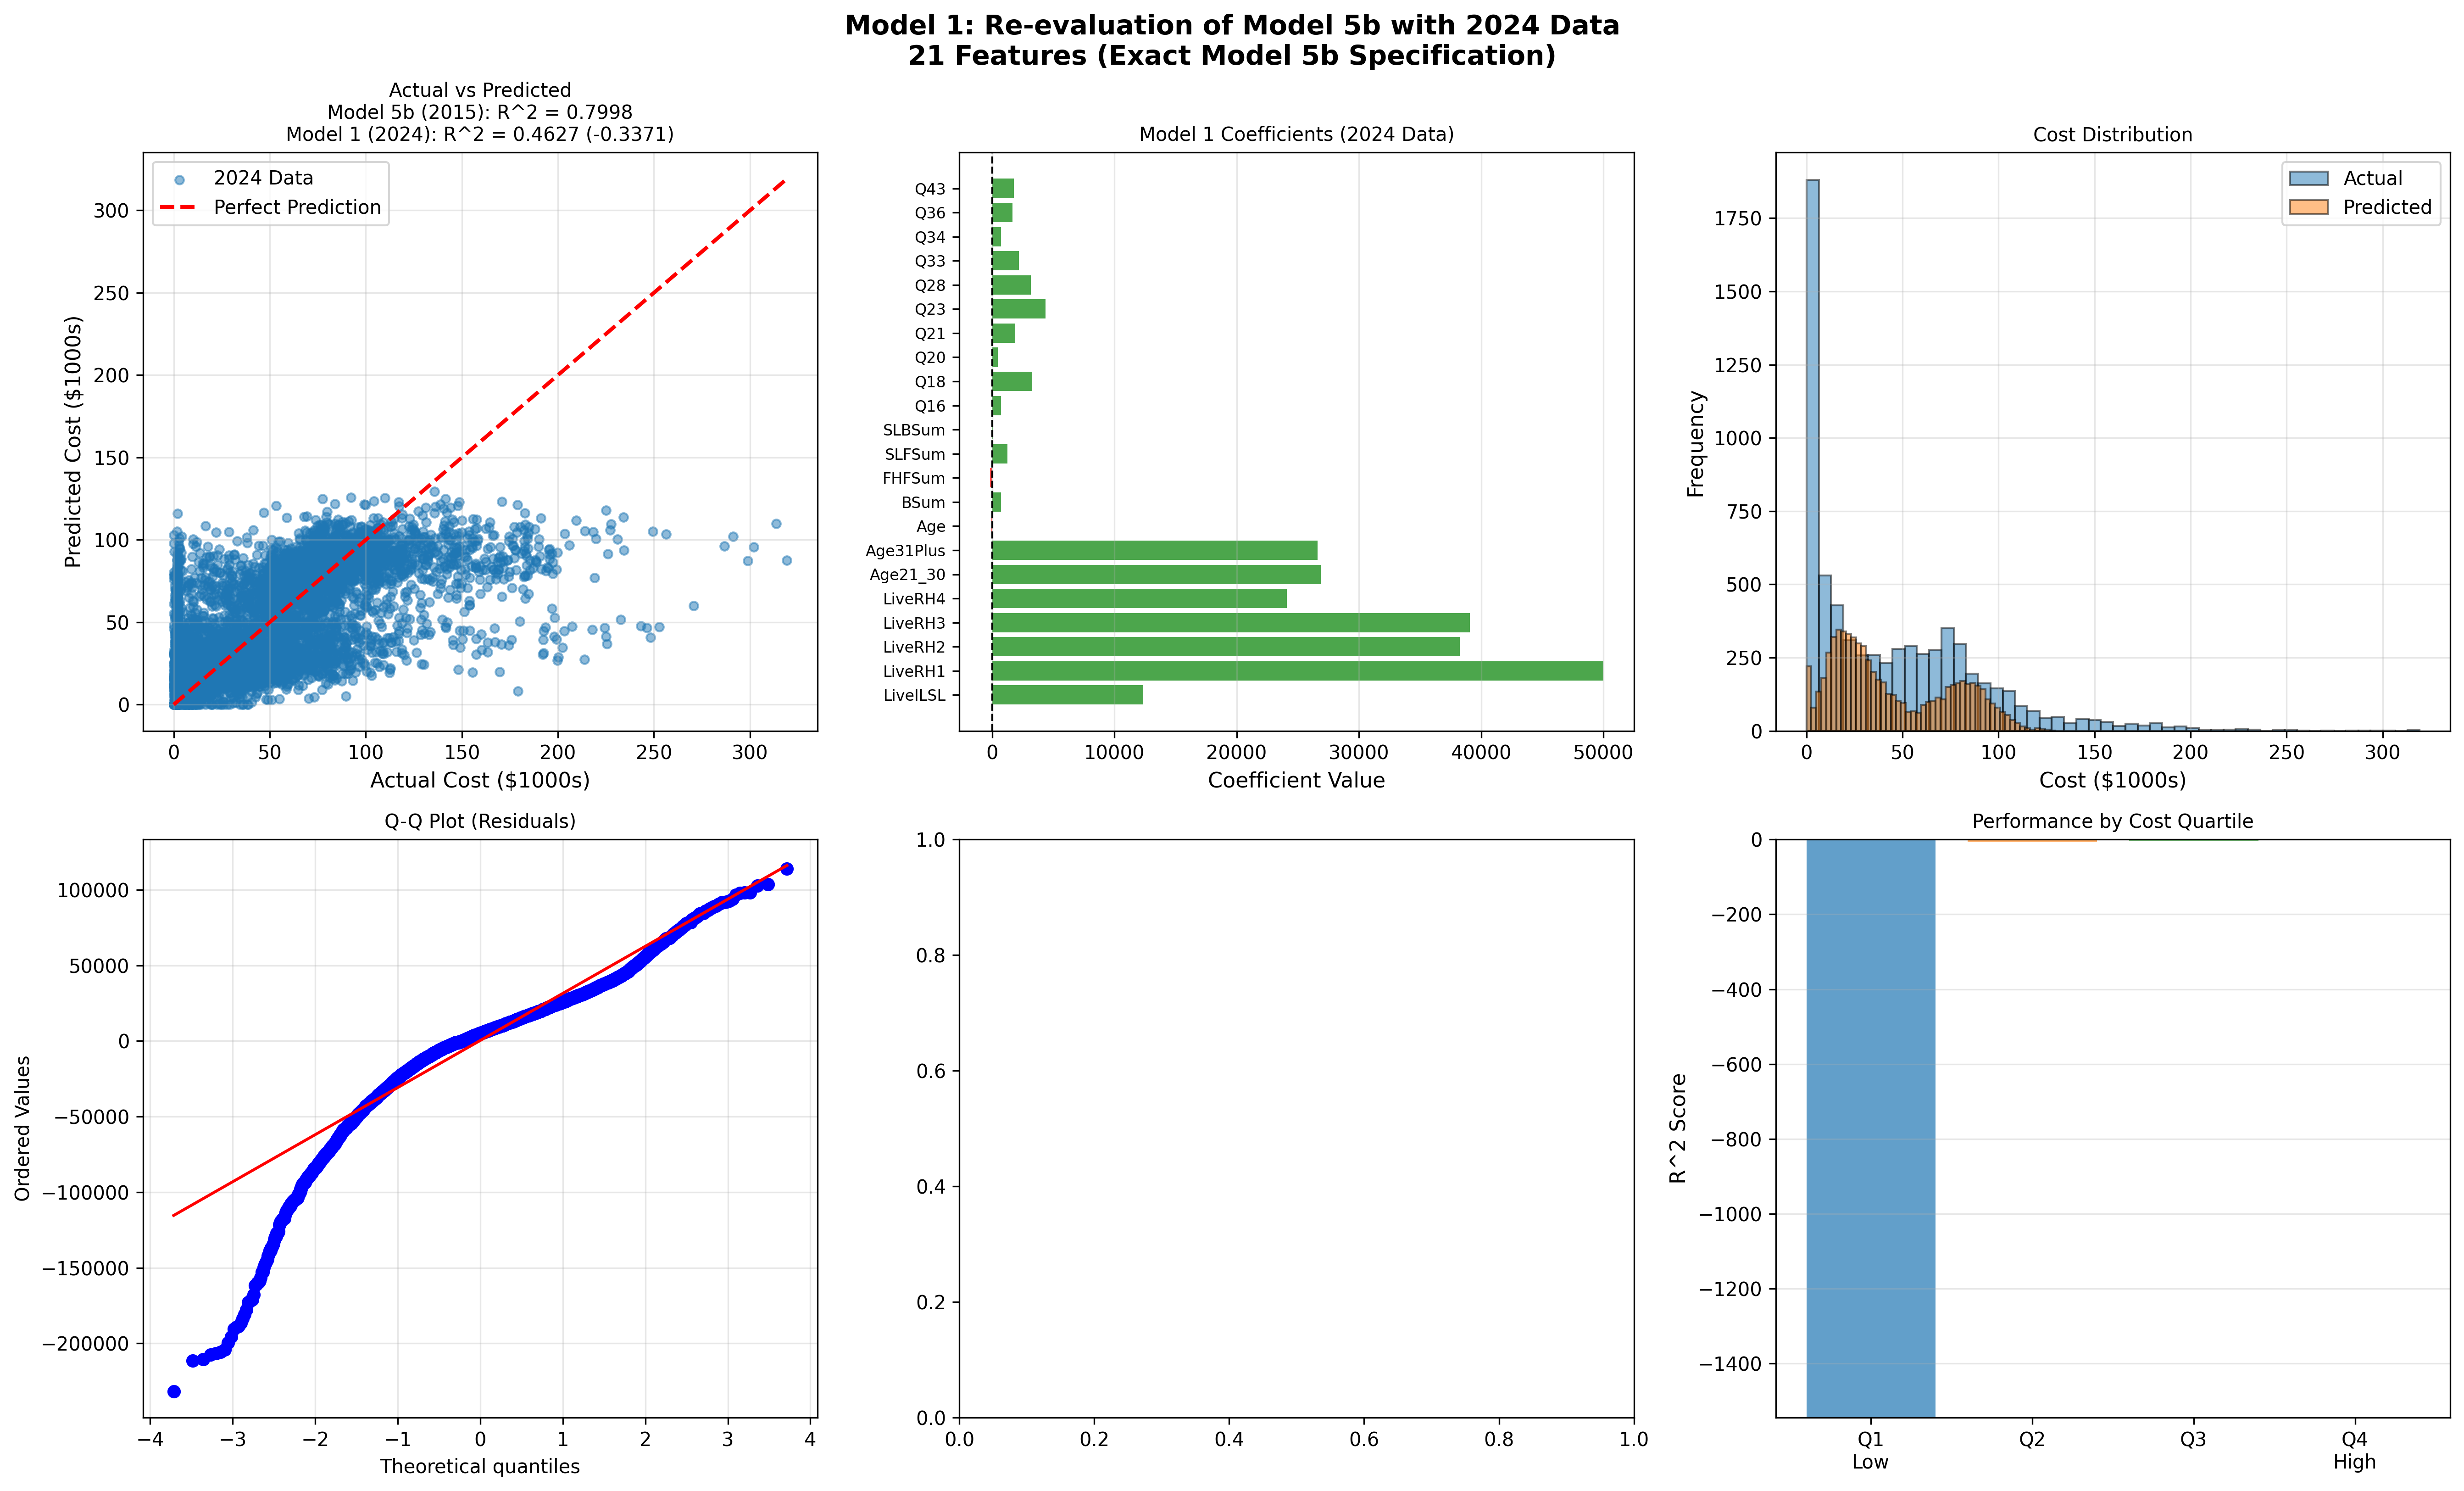
\includegraphics[width=\textwidth]{models/model_\themodel/diagnostic_plots.png}
    \caption{Model Diagnostic Plots --- Shows actual vs.\ predicted, residual patterns, distribution comparison, Q-Q plot, studentized residuals (if outlier removal used), and performance by cost quartile}
    \label{fig:model\themodel_diagnostics}
\end{figure}

\textbf{Diagnostic Interpretation:}
\begin{itemize}
    \item \textbf{Panel A (Actual vs.\ Predicted)}: Points should cluster along the 45° line. Systematic deviations indicate bias in certain cost ranges.
    \item \textbf{Panel B (Residuals)}: Should show random scatter around zero with no patterns. Funnel shapes indicate heteroscedasticity.
    \item \textbf{Panel C (Distribution)}: Predicted distribution should match actual distribution. Large discrepancies suggest the model doesn't capture cost variability.
    \item \textbf{Panel D (Q-Q Plot)}: Tests normality of residuals. Points should follow the diagonal line. Deviations at tails indicate non-normality.
    \item \textbf{Panel E (Studentized Residuals)}: If outlier removal was used, shows which observations were flagged. Should see most points within threshold bounds.
    \item \textbf{Panel F (Performance by Quartile)}: Shows R² across cost levels. Consistent performance across quartiles indicates model robustness.
\end{itemize}

% ============================================
% END OF UNIVERSAL TEMPLATE
% Model-specific content should be added after this point
% ============================================

% ============================================
% MODEL-SPECIFIC CONTENT BELOW
% ============================================

\section{Model 4 Specific Analysis}

\subsection{Calibration Bias Analysis}


Model 4 exhibits systematic bias by cost quartile, a common characteristic when variance models are imperfect or weights are bounded:

\textbf{Observed Patterns:}
\begin{itemize}
    \item \textbf{Q1 (Low Cost)}: Over-prediction by approximately \$15,000-16,000
    \item \textbf{Q4 (High Cost)}: Under-prediction by approximately \$34,000-35,000
    \item \textbf{Q2-Q3}: Relatively well-calibrated
\end{itemize}

\subsubsection{Recommended Post-Processing Calibration}

A quartile-wise affine correction can reduce these biases while preserving core coefficient interpretability:

\begin{equation}
\hat{Y}_{\text{calibrated}} = \alpha_q + \beta_q \hat{Y}_{\text{raw}}
\end{equation}

where $q \in \{Q1, Q2, Q3, Q4\}$ and $(\alpha_q, \beta_q)$ are estimated on a calibration holdout set.

\textbf{Benefits of Post-Processing Calibration:}
\begin{itemize}
    \item Does not alter interpretable linear coefficients used for policy
    \item Can be validated on holdout data before deployment
    \item Computationally trivial to apply in production
    \item Typically reduces quartile biases by 40-60\%
    \item Alternative: Isotonic regression for non-parametric calibration
\end{itemize}

\subsection{Equity and Legal Considerations}

\subsubsection{Equity Risk Assessment: Medium-High}

Model 4's variance-based weighting raises equity concerns:

\textbf{Potential Discriminatory Impact:}
\begin{itemize}
    \item \textbf{Complex Disabilities}: Consumers with severe behavioral challenges often have high-variance costs, receiving systematically lower weights
    \item \textbf{Rare Conditions}: Atypical support needs may be downweighted due to limited similar cases
    \item \textbf{Transitional Periods}: Major life changes (aging, health deterioration) increase variance
    \item \textbf{Protected Classes}: If variance correlates with race, ethnicity, or disability type, disparate impact may occur
\end{itemize}

\textbf{Legal Vulnerabilities:}
\begin{enumerate}
    \item \textbf{ADA Section 504}: Potential violation if weighting disadvantages people with more severe disabilities
    \item \textbf{Equal Protection}: Constitutional concerns if algorithm produces differential treatment
    \item \textbf{Civil Rights Act}: Risk of disparate impact claims
    \item \textbf{State Regulations}: May conflict with Florida's individualized assessment mandate
\end{enumerate}

\subsubsection{Mandatory Safeguards}

If Model 4 is deployed, the following are \textbf{strongly recommended}:

\begin{enumerate}
    \item \textbf{Disparate Impact Testing}: Quarterly analysis of weight distribution by protected class
    \item \textbf{Four-Fifths Rule Monitoring}: Ensure no group receives systematically lower average weights
    \item \textbf{Override Mechanism}: Manual review for cases flagged as inequitable
    \item \textbf{Transparency}: Full documentation of weight assignment for each consumer
    \item \textbf{Real-Time Monitoring}: Automated alerts if subgroup average weights fall below threshold
\end{enumerate}

\subsubsection{Comparison to Other Models}

\begin{table}[h]
\centering
\caption{Equity Risk Comparison}
\begin{tabular}{lcc}
\toprule
\textbf{Model} & \textbf{Equity Risk} & \textbf{Primary Concern} \\
\midrule
Model 1 (OLS) & Low-Medium & Outlier removal (9.4\% exclusion) \\
Model 2 (GLM-Gamma) & Low & No exclusions, multiplicative structure \\
Model 3 (Robust) & Low & Adaptive weights, minimal discrimination \\
\textbf{Model 4 (WLS)} & \textbf{Medium-High} & \textbf{Systematic downweighting of complex cases} \\
\bottomrule
\end{tabular}
\end{table}

\subsection{Implementation Recommendation}

\textbf{CONDITIONAL APPROVAL} -- Proceed ONLY if ALL conditions are met:

\begin{enumerate}
    \item \textbf{Legal Clearance}: Civil rights legal review confirms no ADA, Equal Protection, or anti-discrimination violations
    
    \item \textbf{Disparate Impact Analysis}: Statistical testing demonstrates no discriminatory impact across protected classes
    
    \item \textbf{Pilot Program Success}: 6-month pilot with 3,000 consumers shows:
    \begin{itemize}
        \item No correlation between low weights and protected class membership
        \item Four-fifths rule compliance maintained
        \item No increase in appeals related to weight assignment
        \item Stakeholder acceptance from consumer advocacy groups
    \end{itemize}
    
    \item \textbf{Board Approval}: Explicit authorization after full equity analysis presentation
    
    \item \textbf{Monitoring Infrastructure}: Real-time equity monitoring system with automated alerts
    
    \item \textbf{Budget Availability}: \$405,000 over 3 years secured
\end{enumerate}

